\subsection{Порядок байт}

\begin{frame}
	\tableofcontents[currentsection,currentsubsection]
\end{frame}

\begin{frame}
	Напоминание: порядок бит в байте мы из программы никак не определим, на картинке "--- слева старшие, справа младшие.
	Порядок байт в памяти "--- слева меньшие адреса, справа большие.

	Игра:
	\begin{center}
		\pause
		\begin{tabular}{|c|c|c|c|c|c|c|}
			\hline
			\multicolumn{5}{|c|}{Адрес} & \\\hline
			0 & 1 & 2 & 3 & 4 & Значение \\\hline
			\dots & \dots & \t{0000 0001} & \t{0000 0011} & \dots & \pause 259 \\\hline\noalign{\pause}
			\dots & \dots & \t{0000 0001} & \t{0000 0011} & \dots & \pause 769 \\\hline
		\end{tabular}
		\pause
	\end{center}

	Да как договоримся, так и читать.
	Байты бывают младшие и старшие.
	Договариваются по-разному на разных процессорах и в разных протоколах.
	Свойство <<порядок байт>> называется endianness.
\end{frame}

\begin{frame}

	\begin{center}
		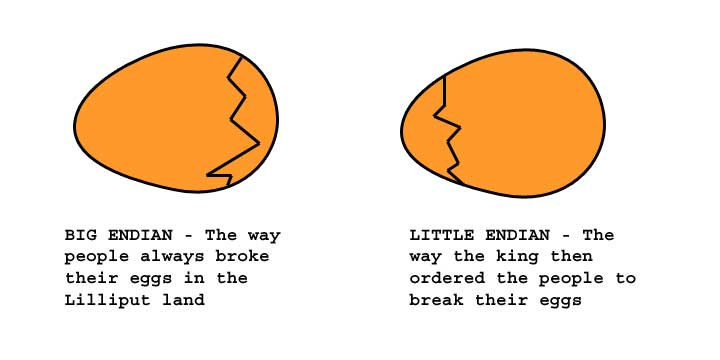
\includegraphics[scale=0.3]{eggs.jpg}
	\end{center}

	Есть два клана: little-endian (остроконечники) и big-endian (тупоконечники).
	По-русски всегда используют английские термины.
\end{frame}

\begin{frame}{Big-endian}
	Используется в низкоуровневых сетевых протоколах (TCP) и процессорах Atmel AVR (ATmega и прочие).

	Младший байт имеет больший адрес.
	Тогда запись совпадает с <<естественной>>:
	\begin{center}
		\begin{tabular}{|c|c|c|c|c|c|c|}
			\hline
			\multicolumn{5}{|c|}{Адрес} & \\\hline
			0 & 1 & 2 & 3 & 4 & Значение \\\hline
			\dots & \dots & \t{0000 0001} & \t{0000 0011} & \dots & $\t{0000 00\textbf{01} 0000 00\textbf{11}}_2=769_{10}$ \\\hline
		\end{tabular}
	\end{center}

	Надо очень аккуратно помнить адрес и размер числа:
	\begin{center}
		\begin{tabular}{|c|c|c|c|c|c|c|}
			\hline
			\multicolumn{5}{|c|}{Адрес} & \\\hline
			0 & 1 & 2 & 3 & 4 & Значение \\\hline
			\dots & \dots & \t{0000 0001} & \dots & \dots & $\t{0000 0001}_2=1_{10}$ \\\hline
		\end{tabular}
	\end{center}
\end{frame}

\begin{frame}{Little-endian}
	Используется в x86.

	Младший байт имеет меньший адрес.
	Читается хуже:
	\begin{center}
		\begin{tabular}{|c|c|c|c|c|c|c|}
			\hline
			\multicolumn{5}{|c|}{Адрес} & \\\hline
			0 & 1 & 2 & 3 & 4 & Значение \\\hline
			\dots & \dots & \t{0000 0001} & \t{0000 0011} & \dots & $\t{0000 00\textbf{11} 0000 00\textbf{01}}_2=259_{10}$ \\\hline
		\end{tabular}
	\end{center}
	Если только мы не Intel и не пишем к этому документацию:
	\begin{center}
		\begin{tabular}{|c|c|c|c|c|c|c|}
			\hline
			\multicolumn{5}{|c|}{Адрес} & \\\hline
			4 & 3 & 2 & 1 & 0 & Значение \\\hline
			\dots & \dots & \t{1100 0000} & \t{1000 0000} & \dots & $\t{0000 0011 0000 0001}_2=259_{10}$ \\\hline
		\end{tabular}
	\end{center}
	Они у себя всё пишут от старших к младшим.
	Получаются байты с меньшими адресами справа.
	И младшие биты справа.
\end{frame}

\begin{frame}{Особенности Little-endian}
	Можно безболезненно конвертировать между типами:
	\begin{center}
		\begin{tabular}{|c|c|c|c|c|c|c|}
			\hline
			\multicolumn{5}{|c|}{Адрес} & \\\hline
			0 & 1 & 2 & 3 & 4 & Значение \\\hline
			\dots & \dots & \t{0000 0011} & \t{0000 0001} & \dots & $\t{0000 00\textbf{11} 0000 00\textbf{01}}_2=259_{10}$ \\\hline
			\dots & \dots & \t{0000 0011} & \dots & \dots & $\t{0000 0011}_2=3_{10}=259_{10} \mod 256$ \\\hline
			\dots & \dots & \t{0000 0101} & \t{0000 0000} & \dots & $\t{0000 0000 0000 0001}_2=5_{10}$ \\\hline
			\dots & \dots & \t{0000 0101} & \dots & \dots & $\t{0000 0001}_2=5_{10}$ \\\hline
			\dots & \dots & \t{1111 0011} & \t{0000 0000} & \dots & $\t{0000 0000 1111 0011}_2=123_{10}$ \\\hline
			\dots & \dots & \t{1111 0011} & \dots & \dots & $\t{1111 0011}_2=123_{10}$ \\\hline
			\dots & \dots & \t{1111 0011} & \dots & \dots & $\t{1111 0011}_2=-133_{10} \mod 256$ \\\hline
			\dots & \dots & \t{1111 0011} & \t{1111 1111} & \dots & $\t{1111 1111 1111 0011}_2=-133_{10} \mod 65536$ \\\hline
		\end{tabular}
	\end{center}
	Ну, почти.
	Со знаками проблема, если мы переходим от меньшего типа к большему.
	Тогда надо расширять знак, если у нас было знаковое число: заполнять старшие байты либо нулями, либо единицами (в зависимости от... \pause старшего бита в числе).
	И даже если беззнаковое, то надо не забыть занулить старшие байты.

	Компиляторы низкоуровневых языков делают это автоматически, когда вы делаете какие-то присваивания.
	Разумеется, надо аккуратно следить за типами, иначе не сделают.

	Привет от функций htons в сокетах.
\end{frame}

\begin{frame}{Резюме}
	\begin{enumerate}
		\item
			Целые числа хранятся в двоичной системе счисления.
		\item
			Знаковость числа определяется лишь типом данных.
		\item
			Самый распространённый способ кодирования отрицательных чисел "--- <<дополнительный код>>.
		\item
			В дополнительном коде старший бит отвечает за знак, а операции сложения/вычитания/умножения делаются абсолютно так же, как и в беззнаковых числах.
		\item
			Операциям сравнения чисел на меньше/больше и делению важно знать, работаем ли мы в дополнительном коде или с беззнаковыми числами.
		\item
			Порядок байт в числах может отличаться даже в разных местах внутри одного приложения.
			Читайте документацию, если работаете с чем-то на уровне байт!
		\item
			Если работаете с little-endian и меняете количество байт в числе "--- позаботьтесь о знаке.
		\item
			Количество бит/байт в числе важно при вычислениях, если есть либо дополнительный код, либо переполнения.
	\end{enumerate}
\end{frame}
